% Tipo de documento (presentación)
\documentclass[usenames,dvipsnames]{beamer}

% Cargar el tema
\usetheme{metropolis}

% Configuración de LaTeX
\usepackage[spanish]{babel}
\usepackage[utf8]{inputenc}

\usepackage{listings}


\usepackage{graphicx,wrapfig,lipsum}

% Configuración básica del tema
\metroset{
  % tema oscuro ('dark') o claro ('light'). No tiene efecto al usar la
  % paleta de colores más adelante
  background=light,
  % 'none' para eliminar la diapositiva inicial de cada sección
  sectionpage=progressbar,
  % 'progressbar' o 'simple' para añadir una diapositiva inicial a cada subsección
  subsectionpage=none,
  % contador de página: 'none', 'counter' o 'fraction'
  numbering=none,
  % barra de progreso: 'none', 'head', 'frametitle' o 'foot'
  progressbar=frametitle,
  % fondo de los bloques estilo teorema: 'transparent' o 'fill'
  block=fill,
}


% Paleta de colores
\definecolor{accent}{RGB}{151, 186, 88}
\colorlet{darkaccent}{accent!70!black}
\definecolor{foreground}{RGB}{0, 0, 0}
\definecolor{background}{RGB}{255, 255, 255}

% Insertar los colores en el tema
\setbeamercolor{normal text}{fg=foreground, bg=background}
\setbeamercolor{alerted text}{fg=darkaccent, bg=background}
\setbeamercolor{example text}{fg=foreground, bg=background}
\setbeamercolor{frametitle}{fg=background, bg=accent}

\setbeamercolor{headtitle}{fg=background!70!accent,bg=accent!90!foreground}
\setbeamercolor{headnav}{fg=background,bg=accent!90!foreground}
\setbeamercolor{section in head/foot}{fg=background,bg=accent}

%
\defbeamertemplate*{headline}{miniframes theme no subsection}{
  % Caja para mostrar título y autor encima de cada diapositiva
  % Nosotros no 
  %% \begin{beamercolorbox}[ht=2.5ex,dp=1.125ex,
  %%     leftskip=.3cm,rightskip=.3cm plus1fil]{headtitle}
  %%   {\usebeamerfont{title in head/foot}\insertshorttitle}
  %%   \hfill
  %%   \leavevmode{\usebeamerfont{author in head/foot}\insertshortauthor}
  %% \end{beamercolorbox}
  %% \begin{beamercolorbox}[colsep=1.5pt]{upper separation line head}
  %% \end{beamercolorbox}

  % Caja para mostrar navegación encima de cada diapositiva
  \begin{beamercolorbox}{headnav}
    \vskip2pt\insertnavigation{\paperwidth}\vskip2pt
  \end{beamercolorbox}
  \begin{beamercolorbox}[colsep=1.5pt]{lower separation line head}
  \end{beamercolorbox}
}

%eye-candy; sintasix más bonita
\newcommand{\seccion}[1]{\input{./sections/#1}}
\newcommand{\foo}{\hspace{-2.3pt}$\bullet$ \hspace{5pt}}

%Meta
\title{Ethereum}
\subtitle{Una nueva visión de la cadena de bloques}
\date{\today}
\institute{Universidad de Granada}
\author{Ana Peña\\Pedro Bonilla}
\titlegraphic{\hfill
\includegraphics[height=1.5cm]{./images/logo.png}}


\begin{document}
\maketitle
\begin{frame}{Contenidos.}
  \setbeamertemplate{section in toc}[sections numbered]
  \tableofcontents [hideallsubsections]
\end{frame}

\section{ Introducción. }
\subsection{intro} %Ponemos la subseccion para que nos aparezcan los circulos de progesion
\begin{frame}{Objetivo.}
	Tras el boom de las cadena de bloques, las criptodivisas simples quedaban cortas y, con el objetivo de dar más funcionalidad a esta tecnología, nació ethereum.
\end{frame}

\begin{frame}{ Historia. }
\scalebox{1}{
\begin{tabular}{r |@{\foo} l}

2014 & WhitePaper de Vitalik Buterin. \\
2014 & Crowdfounding.\\
2015 & Lanzamiento de la plataforma.\\
2016 & Desastre de la DAO.\\
2016 & Nace Ethereum classic.\\
2016 & Dos hard-fork más.\\
2017 & Refuerzo de la seguridad.\\
2017 & Prohibición de las ICO en China.\\
2017 & Exposición de Fundamentos de Redes\\

\end{tabular}}
\end{frame}

\section{ Ethereum. }
\subsection{ethereum. }
\begin{frame}
	Una vez vemos el objetivo que tiene este sistema, vamos a profundizar en detalles de su funcionamiento,
\end{frame}

\begin{frame}{ Bitcoin como sistema de transición de estados. }
Podemos ver el la cadena como un sistema de transición de estados. Esto Seá importante para ver las posibilidades de esta entidad.
\begin{itemize}
	\item Los estados serían el conjunto de la información escrita en cada bloque.
  	\item Tendríamos una  función de transicion: $ APPLY( S , TX ) \to S'\ o\ ERROR$
\end{itemize}
\end{frame}


\begin{frame}{ Bitcoin como sistema de transición de estados. }
Ejemplifiquemos el uso de este sistema.
\begin{itemize}
	\item $ APPLY( \{ Ana: 50 , Pedro: 50 \} , \text{''enviar 20 de Ana a Pedro" )} $
  { Ana: 30 , Pedro: 70 }
  \item  $  APPLY( { Ana: 50 , Pedro: 50 } , \text{''enviar 70 de Ana a Pedro" )} $
  ERROR
\end{itemize}
\end{frame}


\begin{frame} {Cadena de bloques.}
Una cadena de bloques es una base de datos distribuida, formada por cadenas de bloques
diseñadas para evitar su modificación una vez que un dato ha sido publicado usando un sistemabasado en el tiempo y el consenso de los usuarios de esta.\\
\vspace{0.3cm}
\includegraphics[height=2.5cm]{./images/bcn.png}
\end{frame}

\begin{frame}{ Cuentas. }
	Las cuentas son las entidades base de ethereum, y contiene 4 campos:
	\begin{itemize}
	\item Nonce.
	\item Valor.
	\item Código de Contrato.
	\item Almacenamiento.
	\end{itemize}
\end{frame}


\begin{frame}{ Máquina Virtual de Ethereum . }
Con ethereum, cada vez que se usa un programa, una red de miles de computadores lo procesa. 
\includegraphics[width=\textwidth]{./images/EVM.png}\\Los contratos escritos en un lenguaje de programación específico de contrato inteligente se compilan en ‘bytecode’, lo que una prestación llamada ‘ethereum virtual machine’ (EVM) puede leer y ejecutar.
\end{frame}

\begin{frame}{ Mensajes, Transacciones y estado de transición. }

Los mensajes en ethereum son parecidos de cierto modo a las transacciones de en otros  sistemas de cadena de bloques, pero  con algunas caracteristicas llamativas. Un mensaje puede ser creado tanto por una entidad externa como por un contrato, los mensajes pueden contener datos o, si el mensaje es recibido por un contrato, este tiene la opcion de responder. Esto implica que un mensaje en etherum puede toar el aspecto de función.\\
\end{frame}


\begin{frame}{ Contratos inteligentes. }
Un contrato inteligente (en inglés Smart contract) es un programa informático que facilita, asegura, hace cumplir y ejecuta acuerdos registrados entre dos o más partes (por ejemplo personas u organizaciones). Como tales ellos les ayudarían en la negociación y definición de tales acuerdos que causarán que ciertas acciones sucedan como resultado de que se cumplan una serie de condiciones específicas.\\
\end{frame}

\begin{frame}{ Minería y Prueba de Trabajo. }
	
La minería juega un papel importante en asegurarse como funciona ethereum, pero de forma subliminal. Además del objetivo de generar nuevos ether sin la necesidad de un banco, pero esta no es su único rol. Normalmente, es la compañía que centraliza las operaciones (como un banco) la que se asegura de mantener resgistros adecuados de los datos. Sin embargo, los sistemas de cadena de bloques introducen una nuevo modo de mantener el resgistro de acciones, cuando es la red entera la que se asegura de mantener el registro de transacciones, en lugar de un intermediario, y las anota en un registro público.\\
\begin{center}
\hfill\includegraphics[height=1.5cm]{./images/miner.png}
\end{center}
\end{frame}

\begin{frame}{ Hardfork y Sotfork. }
El término fork hace referencia al despliegue de cambios en el código de la cadena de bloques. La bifurcaión sucede cuando el equipo detras de ethreum quiere implantr cambios en la estructura por diversos motivos. Como la cadena de bloques es una estructura de datos descentralizada, hay diferentes, esto provoca que estas situcaciones generen cadenas de bloques alternativas. Es lo que se conoce como bifurcación de la Blockchain, y aquí es donde entran en juego los conceptos de hardfork y softfork.\\
\end{frame}


\section { Aplicaciones. }
\subsection{aplicaciones. }

\begin{frame}{ Sistemas de Token. }
	
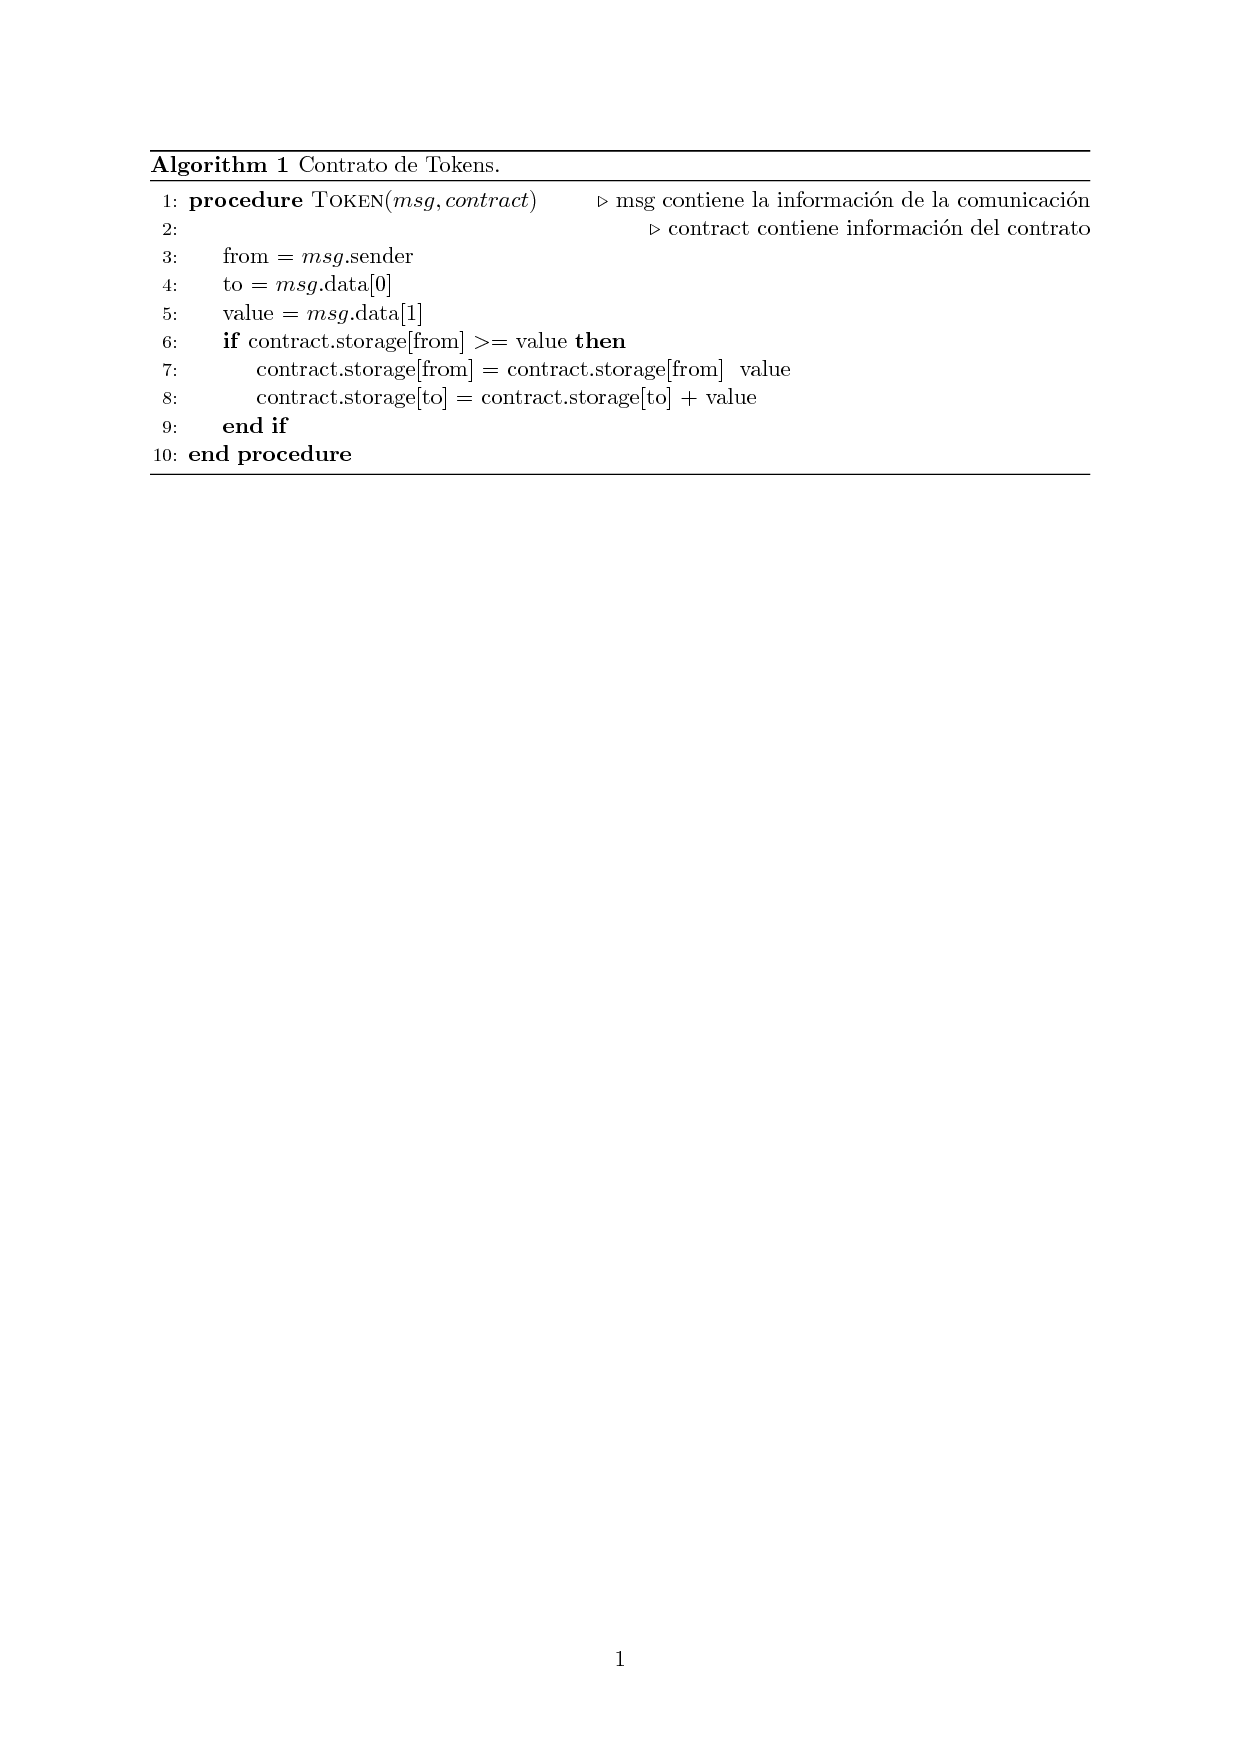
\includegraphics[width=\textwidth]{./images/alg1.png}
\end{frame}
\begin{frame}{ Sistema de identidad. }

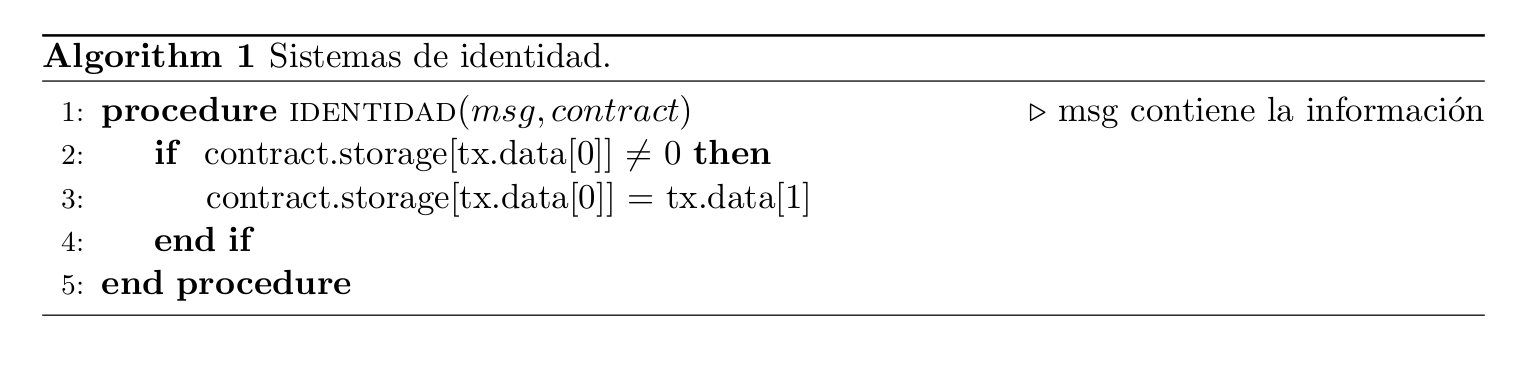
\includegraphics[width=\textwidth]{./images/alg2.png}
\end{frame}
\begin{frame}{ Más aplicaciones. }
	¡En el github \url{https://github.com/pedrobn23/Ether} tenemos más, mirenlo para profundizar vuestro saber!
\end{frame}

\section{ Particularidades. }
\subsection{Particularidades}

\begin{frame}{ Ether. }

	\begin{columns}
   \column{.5\textwidth}
Aunque nadie sea dueño de ethereum, el sistema que respalda esta funcionalidad no es gratis. Mejor dicho, la red necesita el ‘ether’, una pieza única de código que puede usarse para pagar por los recursos computacionales necesarios para ejecutar una aplicación o programa. El ether no es más que la divisa utilizada en ethereum para las transacciones.

   \column{.5\textwidth}
   
\includegraphics[width=0.9\textwidth]{./images/ETH-512.png}

\end{columns}

\end{frame}

\begin{frame}{ DoS attack. }
	En el pasado se han visto problemas con la capacidad de ethereum para soportar este tipo de ataques, por ejemplo en la compañía \underline{bancor}. Estos problemas están relacionados con la capacidad de escalabilidad de ethereum. Por ello, vamos a explicar en que consiste este tipo de ataques.\\
	\url{https://motherboard.vice.com/en_us/article/newk7m/the-ethereum-network-is-ddos-ing-itself}
\end{frame}

\begin{frame}{ Escalabilidad. }
	\begin{columns}
   \column{.5\textwidth}

\includegraphics[width=\textwidth]{./images/scalability.png}

   \column{.5\textwidth}
   
Una preocupación común acerca de Ethereum es el tema de la escalabilidad. Ethereum sufre el defecto de que cada transacción tiene que ser procesada por cada nodo en la red.

\end{columns}

\end{frame}
\begin{frame}{ Minería centralizada .}
Actualmente, las dos mining pools principales indirectamente controlan aproximadamente el 50\% del poder de procesamiento en la red de Bitcoin, aunque esto está mitigado por el hecho de que los mineros pueden cambiarse a otras mining pools si una pool o coalición pretende llevar a cabo un \underline{\textbf{ataque del 51\%}}. El propósito actual en Ethereum es usar un algoritmo de minería basado en generar aleatoriamente una única función hash por cada 1000 ‘nonces’, usando un rango de computación lo suficientemente amplio para eliminar el beneficio del hardware especializado.

\end{frame}
\section{Conclusiones}
\subsection{Conclusiones}
\begin{frame}[standout]
  ¡Muchas gracias!
\end{frame}
\end{document}
\end{document}
